\documentclass{sigchi}

% Use this command to override the default ACM copyright statement (e.g. for preprints). 
% Consult the conference website for the camera-ready copyright statement.
%% \toappear{
%% Permission to make digital or hard copies of all or part of this
%% work for personal or classroom use is granted without fee provided that 
%% copies are not made or distributed for profit or commercial advantage and
%% that copies bear this notice and the full citation on the first page. To
%% copy otherwise, or republish, to post on servers or to redistribute to 
%% lists, requires prior specific permission and/or a fee.\\
%{\confname{CHI'13}}, May 5--10, 2012, Austin, Texas, USA.\\
%Copyright 2012 ACM 978-1-4503-1015-4/12/05...\$10.00.
%}

% Arabic page numbers for submission. 
% Remove this line to eliminate page numbers for the camera ready copy
%\pagenumbering{arabic}


% Load basic packages
\usepackage{balance}  % to better equalize the last page
\usepackage{graphics} % for EPS, load graphicx instead
\usepackage{times}    % comment if you want LaTeX's default font
\usepackage{url}      % llt: nicely formatted URLs

% llt: Define a global style for URLs, rather that the default one
\makeatletter
\def\url@leostyle{%
  \@ifundefined{selectfont}{\def\UrlFont{\sf}}{\def\UrlFont{\small\bf\ttfamily}}}
\makeatother
\urlstyle{leo}


% To make various LaTeX processors do the right thing with page size.
\def\pprw{8.5in}
\def\pprh{11in}
\special{papersize=\pprw,\pprh}
\setlength{\paperwidth}{\pprw}
\setlength{\paperheight}{\pprh}
\setlength{\pdfpagewidth}{\pprw}
\setlength{\pdfpageheight}{\pprh}

% Make sure hyperref comes last of your loaded packages, 
% to give it a fighting chance of not being over-written, 
% since its job is to redefine many LaTeX commands.
\usepackage[pdftex]{hyperref}
\hypersetup{
pdftitle={SIGCHI Conference Proceedings Format},
pdfauthor={LaTeX},
pdfkeywords={SIGCHI, proceedings, archival format},
bookmarksnumbered,
pdfstartview={FitH},
colorlinks,
citecolor=black,
filecolor=black,
linkcolor=black,
urlcolor=black,
breaklinks=true,
}

% create a shortcut to typeset table headings
\newcommand\tabhead[1]{\small\textbf{#1}}


% End of preamble. Here it comes the document.
\begin{document}

\title{Carp\'{e} Data: Supporting Serendipitous Data Integration in Personal Information Management}

\numberofauthors{3}
\author{
  \alignauthor 1st Author Name\\
    \affaddr{Affiliation}\\
    \affaddr{Address}\\
    \email{e-mail address}\\
    \affaddr{Optional phone number}
  \alignauthor 2nd Author Name\\
    \affaddr{Affiliation}\\
    \affaddr{Address}\\
    \email{e-mail address}\\
    \affaddr{Optional phone number}    
  \alignauthor 3rd Author Name\\
    \affaddr{Affiliation}\\
    \affaddr{Address}\\
    \email{e-mail address}\\
    \affaddr{Optional phone number}
}

% Teaser figure can go here
%\teaser{
%  \centering
%  
\includegraphics{Figure1}
%  \caption{Teaser Image}
%  \label{fig:teaser}
%}

\maketitle

\begin{abstract}
Exploratory sequential mixed-method study
\end{abstract}

\keywords{}

\category{H.5.m.}{Information Interfaces and Presentation (e.g. HCI)}{Miscellaneous}

\terms{Human Factors; Design; Measurement.}

\section{Introduction}

In recent years, an unprecedented quantity and variety of information has been made available as structured data on the Web, through APIs, datasets, and data feeds.  This information includes: access to data previously hidden behind services and applications, such as retailer product catalogues; information not previously directly released to the public, such as open government data or records of personal financial transactions; and new kinds of data generated by emerging kinds of data sources, such as wearable and smartphone-based biosensors.  A primary goal of opening up such direct access to information is that end-user citizens will make more informed decisions pertaining to their personal information, for example health, wealth, and well-being \cite{}.  This data is predominately used by  specialised app developers, journalists and other ``data specialists'' but remains inaccessible to citizens because of the available tools.  For example, the most commonly used structured personal information management (PIM) tools either manage a small, fixed set of data types (such as digital calendaring tools and  to-do list managers) or provide little or no support for structured data at all, such as text editors and sketching/drawing tools \cite{}.   

We hypothesise that end-users would benefit from this rich data with tools allowing them to effectively browse, use and consume heterogeneous structured data from diverse sources.  In this paper, we present our investigation of how extending PIM tools to effectively use emerging ecosystems of personal data impact information practice.  We used a three stage sequential exploratory mixed-method approach: first, we performed a qualitative analysis of a semi-structured interview pre-study to understand the types of tasks people performed using a plurality of  information sources, and the processes that they relied upon to perform such tasks.  Our results suggested that people preferred to rely upon multiple, diverse sources to singular, integrated ones for a number of reasons, including coverage, reliability, and seeking out more suitable alternatives.  

Second, we conducted a quantitative, structural analysis of various popular personal data sources available today to identify potential barriers to effective unification of data from each.  Drawing upon definitions from the database integration and automatic schema matching literature, we characterised the types of heterogeneity exhibited across data sources in three popular domains: social networking, shopping, and dining, finding that terminological heterogeneity dominates the simpler data feeds (including social networking and restaurant recommendations), while structural issues pervade the more complex schemas of online retailers' product catalogues.

Third, we developed DataPalette, which focuses on the most common types of heterogeneity to enable serendipitous ``data mixing'' - a form of simple integration sufficient to allow people to easily and effectively combine and compare information sources without the need to write code.  It was principally designed based upon people's data integration needs and to support data heterogeneity observed in the previous studies.  We embarked on a user-centric design exercise towards an interface to facilitate simple, ``light-touch'' integration tasks of diverse, heterogeneous data sources.  We then performed a usability evaluation of DataPalette, which revealed that most users were comfortable with the interactive integration mechanisms we devised, and that this interface effectively improved people's ability to perform multifaceted decision making tasks using multiple sources.

\section{Background}

In this section, we touch on motivating work for DataPalette from three fields: personal information management, data integration, and end-user mashups and toolkits.

The primary motivation for this work stems from field studies in personal information management, where letting users effectively consolidate and work with data from multiple sources has remained a challenge for over a decade. The problem of data fragmentation (\cite{Jones05towardsa}, for example, derives from an inability to effectively consolidate data across multiple applications, services and platforms (e.g., \cite{bergman}, \cite{boardmansasse}). In our own previously-conducted field study, (reference anonymised) we observed variations of manual ``coping strategies'' (or, if programmers, elaborate, custom-coded one-off solutions) to allow people to manage heterogeneous data from disparate sources -- be them online, offline, or other people.  Similar findings from other studies include Voida et al.'s observations of volunteer coordinators' ``homebrew databases'', manually-maintained information assemblages concocted to handle the widely varied and heterogeneous data collection requirements such groups needed to coordinate their activities \cite{Voida:2011:HDC:1978942.1979078}.
%% TODO MORE HERE

%% don't like the beginning of this > 
Enabling PIM tools to supporting ad-hoc data integration has remained difficult because of the complex, theoretically difficult nature of data hetereogeneity; specifically, reconciling the differences that arise among representations when data is created by different people, at different times, for different purposes. As described by Alon Halvey:

\begin{quote} 
  [The problem stems from the fact that] we are trying to integrate data systems that were developed for slightly (or vastly) different business needs. Hence, even if they model overlapping domains, they will model them in different ways. Differing structures are a byproduct of human nature --- people think differently from one another even when faced with the same modeling goal. \cite{alonhalevy}
\end{quote}

% i think we do not need to differentiate between semantic web and databse integration here, we're saying they're both bad, let's lump them together to keep the argument flowing and not kill our readers
The database integration and Semantic Web \cite{Shadbolt:2006:SWR:1155313.1155373} research communities have primarily focused efforts on purely-automatic approaches to the problem of data integration.  Such approaches typically take the form of either \emph{ontology} or \emph{schema-level matching}, or \emph{direct} or \emph{instance-level} matching.  We presently focus  on \emph{instance-level} matching, as schemas may not always be available, nor easily accesssed by users. Approaches to automatic instance matching have included applied natural language processing (NLP) techniques for terminological matching (e.g., \cite{euzenat2004api}), machine-learning techniques that use both structural and terminological features for matching \cite{doan2003learning}, probabilistic approaches \cite{suchanek2011paris}, and instance schema comparisons using structural and logical definitions \cite{castano2006matching}.   In real-world settings, however, manual and semi-automatic matching approaches are favoured over automatic because of the need for high degrees of accuracy.  

A different approach entirely has been taken in the web mash-up community; this community has largely focused on end-user interfaces that allow people to interactively reconcile data from multiple sources.  Yahoo Pipes! is a visual programming language aimed at letting novice programmers easily create data-transformation workflows, but remained rather challenging to  use and effort-intensive for one-off information tasks.  Mash-up makers such as Intel Mashmaker \cite{}, QDEWiki \cite{}, and TX2 \cite{}. DataPalette's approach is most directly inspired by ``lightweight'' visual, user-interactive data collection, consolidation and alignment tools such as Potluck \cite{citeulike:3875264} and Cards \cite{Dontcheva:2007:RCS:1294211.1294224}.

% Semi-automatic approaches use varying levels of support to aid a user, from prompting users to manually check flagged alignments, to suggesting possible alignments.  Allowing users to compare instances across heterogeneous data is powerful because users can combine and evaluate multiple sources.  In principle, automatic instance matching approaches would allow users to seamlessly browse this data, however for now and the foreseeable future such approaches cannot make use of personal knowledge and do not guarantee their alignments.  Therefore, in our work, we adopt a semi-automated matching approach, which will support the user to make alignments between web data and their personal data.

A number of research PIM systems have demonstrated a great number of ways that users could benefit from better support for data integration.  For example, SEMEX's \cite{semex} rich uniform query interface allowed users to quickly trace references of people, places and things across files, folders and repositories.  Similarly, Haystack, a personal information platform, allowed users to visualise and customise how they worked with their data in a uniform, consolidated manner \cite{haystack}. Pertaining to each system's ability to integrate information from arbitrary new data sources, however, both systems generally required new sources to either already conform to a pre-specified set of ontologies, or have the user provide a manual specify such a mapping translation themselves.


% integrated into the above :: 

%% The Semantic Web research community has approached the problem of data integration in terms of \emph{ontology matching}, which can be split into two distinct strategies: \emph{schema} and \emph{instance} matching.  Instance matching differs from schema level matching in that it aims to detect instances referring to the same real world object, while schema matching aims to find a set of mappings between concepts and properties in different ontologies. For our purposes of allowing users to explore and compare data from different websites, we are particularly interested in aligning instances of the most common forms of data that people compare from website to website.  
%% Instance matching within this scope is in its infancy, some of its problems have been addressed by the record linkage problem in the database field \cite{fellegi1969theory,winkler1999state,gu2003record}.  However, there are new problems to address in this field, which are strongly related to schema matching, including structural heterogeneity and logical heterogeneity. The approaches used to match instances typically use: natural language processing, using lexicons like Wordnet\footnote{\emph{Wordnet} - \url{http://wordnet.princeton.edu}} to identify synonyms, and word stems \cite{euzenat2004api}; machine learning techniques \cite{doan2003learning}; probabilistic approaches \cite{suchanek2011paris} and comparisons of instance schemas structural and logical definitions \cite{castano2006matching}.  In our case, this is problematic because information from the web does not always have a schema.  In real-world scenarios, semi-automatic ontology matching approaches are favoured over automatic because reconciling the differences between ontologies that were designed for different purposes is not always accurate.  Semi-automatic approaches use varying levels of support to aid a user, from prompting users to manually check flagged alignments, to suggesting possible alignments.  Allowing users to compare instances across heterogeneous data is powerful because users can combine and evaluate multiple sources.  In principle, automatic instance matching approaches would allow users to seamlessly browse this data, however for now and the foreseeable future such approaches cannot make use of personal knowledge and do not guarantee their alignments.  Therefore, in our work, we adopt a semi-automated matching approach, which will support the user to make alignments between web data and their personal data.
%% The Semantic Web community use ontologies to formally describe vocabularies for specific domains by defining axioms describing entities, instances of entities and the relationships that hold among them \cite{borst1997construction}. The axioms in an ontology can be either assertional or terminological, the former describes the schema of the entities and the latter the instances of those entities. Typically, these ontologies are marked up using OWL (Web Ontology Language) and Resource Description Framework Schema (RDF(S)).  There has been an explosion of ontologies published online, many of which describe the same entities.  These entities may or may not share the same entity names or properties.  Therefore using data from heterogeneous ontologies can be difficult. The field of ontology matching can be split into two fields: schema and instance matching.  Instance matching differs from schema level matching, because it aims to detect instances referring to the same real world object, while schema matching aims to find a set of mappings between concepts and properties in different ontologies.
% For our purposes of allowing users to explore and compare data from different websites, we are particularly interested in aligning instances of the most common forms of data that people compare from website to website.  Instance matching within this scope is in its infancy, some of its problems have been addressed by the record linkage problem in the database field \cite{fellegi1969theory,winkler1999state,gu2003record}.  However, there are new problems to address in this field, which are strongly related to schema matching, including structural heterogeneity and logical heterogeneity.
% The approaches used to match instances typically use: natural language processing, using lexicons like Wordnet to identify synonyms, and word stems \cite{euzenat2004api}; machine learning techniques \cite{doan2003learning}; probabilistic approaches \cite{suchanek2011paris} and comparisons of instance schemas structural and logical definitions \cite{castano2006matching}.  In our case, this is problematic because information from the web does not always have a schema.  In real-world scenarios, semi-automatic ontology matching approaches are favoured over automatic because reconciling the differences between ontologies that were designed for different purposes is not always accurate.  Semi-automatic approaches use varying levels of support to aid a user, from prompting users to manually check flagged alignments, to suggesting possible alignments.  Allowing users to compare instances across heterogeneous data is powerful because users can combine and evaluate multiple sources.  In principle, automatic instance matching approaches would allow users to seamlessly browse this data, however for now and the foreseeable future such approaches cannot make use of personal knowledge and do not guarantee their alignments.  Therefore, in our work, we adopt a semi-automated matching approach, which will support the user to make alignments between web data and their personal data.

\section{Pre-studies: The Need for and Challenges in realizing Ad-Hoc Data Integration in PIM Tools}

%% not sure where this goes >> but i want to keep it

We performed an exploratory sequential mixed-method study to help us design our contribution. For our first pre-study, we first sought an updated understanding of how and whether people still used multiple information sources regularly when they sought information on the Web. There were several reasons for this inquiry; first, we wondered whether people were increasingly relying only on the handful of the massive ``supersites'' (Facebook, Google, Wikipedia) for most of their activities, instead of  searching across distributed sources of information.  If this were the case, much of the benefit could be gained by merely integrating PIM tools with the handful of sites, rather than the substantially more challenging problem of integrating data from arbitrary information sources on the Web.   Second, if people did rely on multiple sites, we wished to know why, and the typical kinds of tasks people did that required diverse information collection - were these kinds of tasks rare?  If so, this would suggest that perhaps specialised interfaces could be concocted for this purpose rather than it being a PIM need. 

The second pre-study focused on the characteristics of the data available from the kinds of sites used by the first pre-study's participants for the tasks described. The purpose of this follow-on  was to identify not specific characteristics of particular sites in question, but to identify, in general, the degree of complexity of the data feeds currently available across a variety of domains, and typical integration problems that might arise when mixing this data. In the remaining part sof this section, we summarise our methodologies and results for each of these two pre-studies.


\subsection{PS.1 - Understanding Data Diversity in Everyday Tasks}
We designed a semi-structured interview about tasks people performed online that required the use of multiple websites, and the processes people used to perform such tasks.  We analysed the data collected from this study using a thematic approach, as described below. 

Our pre-study investigated the types of tasks people performed online that required heterogeneous data sources, and which tools they would use to organise a large social event involving 15 or more people.  We interviewed 8 participants, using a general interview guide approach based loosely on a set of questions.  This approach allowed both the participant and interviewer a degree of freedom in conversation and each interview could adapt to the participant's experiences, while collecting the same general areas of information.  Each interview was recorded and notes taken, the interviewer was trained so that they were knowledgeable about the importance of the study and to minimise bias.

\subsubsection{Results}
The participant demographic consisted of 8 people, 7 of which were male and 1 female.  They were split evenly into two age groups of 18-25 and 26-32.  All but one participant reported they used social network sites very regularly (many times a day); they said they either logged in multiple times a day, left a website page open or used dedicated application for their social networking site updates.  Those that used social networking websites primarily used Facebook.  All of the participants used Twitter to listen to broadcasted tweets, and 6 out of 8 people regularly tweeted. 

\subsubsection{Question 1: Tasks}
All participants reported having used multiple websites to accomplish a task.  They listed example tasks such as shopping (including food, consumer electronics, hotels and flights), searching for jobs, choosing recipes, study and work.  The biggest focus for shopping focused tasks was balancing price, quality and speed of delivery.  In general, people did not not trust a single websites for reviews because they said that they could be biased and did not always review the features they were interested in.  One participant said that video reviews of items were really important because they showed the aesthetics and scale of the item.  In general for initial research into organising a task it was typical to Google keywords to find related websites to their tasks.  They identified that they used different website for different jobs, such as manufacturers website for technical details, review aggregators for a range of opinions, and Google maps for location based decisions.  Social networks were also identified to have different functions, such as different groups of people belong to each and share different types of opinions.  One participant said that they shared their outlook and gmail calendars, but only for work events and did not record social activities on them.

\subsubsection{Question 2: Process Used to Organise a Large Social Event}
All of the participants would organise a large social event by talking to their friends, about their ideas, preferences and recommendations.  The tools they would use to acquire this information included face-to-face, phone calls, email, Skype, Facebook events.  The method chosen depended on the time scale required to organise an event, in general if there was a short time scale people would speak in person or on the phone.  Otherwise, people would set up a Facebook event page to discuss ideas with their friends.  If their friends were not on Facebook they would email them.  All but one participant said they would not use Doodle\footnote{Doodle - \emph{www.doodle.com}} to organise day and time of an event, because they felt that people did not fill in the form and it was more suit to organising work event not social.  

Most people felt that being assertive and posting their decisions about the date and time on Facebook meant that organising events were more successful than trying to gather a consensus.  They expected that their friends would voice any objections if they could not attend or like the restaurant or activity selected.   They selected venues, locations, restaurants and activities based on their own knowledge, friend's recommendations, Google maps, reviews obtained through web search and sites such as tripadvisor.  People stated that the cost, price and easy to get to locations were the most important factors when choosing a venue.  They considered how to get there and looked up train or bus times on the Web.  One participant organised carpools informally and at last minute via Facebook or text messages.

When organising an event the weather was not that important because it they did not trust its accuracy for events plan further in the future than one week.  Also, their friend's preferences in price and food choices were not a priority; they would try to be inclusive but only if it meant small changes to the plan.  Choosing food and timings were often made on-the-fly, by either with the use of mobile applications or by walking past a location.

\subsubsection{Summary of Findings}
People said that they would like a website that could support the evolution of an event, that allowed them to post drafts of an event.  They felt that organising an event should be a process that changes over time and did not need rushing.  Three of the participants said that they would like a recommendation system for places to eat and activities. Another strong requirement was that it had to be ubiquitous so that everyone could use it because they wanted a single place to communicate with their friends.  While Facebook was the most popular social networking site for organising events, half of the participants felt that it was not the best solution and would prefer a collaborative environment, which could be wiki based.


%% TODO THIS IS PLACEHOLDER DATA >> 
\begin{table*}
\small
\begin{tabular}{| p{2.0cm} | p{1.5cm} | p{3.6cm} | p{2cm} | p{2cm} | l | l | l | l |}
\hline
source category  & data type & sources & API type & avg fields/rec & avg depth & term. & struct & semantic \\
\hline
social networking  & person's profile & Facebook, LinkedIn, Google+ & REST (JSON/XML) & 10 & 1.2 & 0.90 & 0.10 & 1.0 \\
event calendars & events & Eventbrite, Google Calendar  & REST (JSON/XML) & 10 & 1.2 & 0.90 & 0.10 & 1.0 \\
retail (shopping)  & product profile & Amazon, Shopping.com, Etsy, Groupon, Zappos  & REST (JSON/XML) & 10 & 1.2 & 0.90 & 0.10 & 1.0 \\
music catalogues & songs and albums & Echonest, rdio, Soundcloud, Spotify  & REST (JSON/XML) & 10 & 1.2 & 0.90 & 0.10 & 1.0 \\
weather & forecasts & W.Underground, Weatherbug, Yahoo! Weather & REST (JSON/XML) & 10 & 1.2 & 0.90 & 0.10 & 1.0 \\
\hline
\end{tabular}
\caption{\emph{PS.2 Results} - Analysis of heterogeneity present across data feeds, by category of feed}\label{tbl:prestudy2}

\end{table*}
%% << 

\subsection{PS.2 - Technical Challenges of Data Integration}
Our investigation of integration challenges started with identifying a set of candidate data sources for analysis.  For this, we consulted the ProgrammableWeb API directory\footnote{ProgrammableWeb - \url{http://www.programmableweb.com/apis/directory}} of 50 most popular data feeds measured by the number of developer API keys issued for each.  In order to get a variety of different kinds of sources represented, we first categorised feeds into 5 topic categories: social networks (people), retail (shopping), events (calendar events, happenings, etc), music, and weather. We then populated each category with 2-5 feeds each depending on feed availability, for a total of 15 total feeds.  

For each feed, 3-5 data records were obtained by querying the API directly for records using popular key terms for each category's primary \emph{corresponding type}, listed in the second colum of Table \ref{tbl:prestudy2}. While many of the APIs also provided access to other kinds of data, such as customer reviews, only the primary type were obtained for each category; e.g., product records for the \emph{shopping} category.  Once data records were obtained, two complexity metrics were computed for each, followed by pairwise heterogeneity metrics.  Since, due to optional fields,  individual records could vary in the number of fields.  An alternative approach to using instance documents was to directly compare schema definitions directly; however, this approach was abandoned after an initial investigation revealed two problems with schema analysis.  First, many of the sites' schema documentation was not actually publicly available; second, that many of the schemas were not actually representative of typical data returned by the service. For example, the schema documentation for \emph{shopping.com} listed full product attribute properties, but none of the records actually returned for the products we queried contained such attributes. 

The per-source metrics were as follows:
\begin{itemize}
\item \emph{Average Width of record} - Average number of properties per record.
\item \emph{Average Depth of record} - Average depth of data record (number of subproperties in self-contained record). (In JSON/XML representations, this is the tree depth; for RDF  representations this is merely the number of embedded entity resource definitions included in the top-level query).
\end{itemize}

Heterogeneity was measured through \emph{pairwise consistency metrics} we derived from definitions in \cite{george2005understanding} and feature-metrics used in statistical instance alignment algorithms (such as summarised in \cite{bhattacharya2007collective}). Such metrics were chosen because they reflected, the differences among the data feeds at multiple levels - from the simple (labelling) differneces to differences in how data was structured, and modeled. Each such metric listed above is the result of averaging the pairwise score between sources in each category, separately and defined as follows:

\begin{itemize}
\item \emph{Terminological consistency} - Percent of property names that match
\item \emph{Structural consistency} - Percent of properties that have \emph{compatible structures}
\item \emph{Semantic/Model consistency} - Percent of entities/concepts that have corresponding fields 
\item \emph{Value consistency} - Percent of values that are compatible
\end{itemize}

\subsubsection{Results}
% TODO TODO TODO TODO 
Our findings suggest that 

\section{Designing DataPalette : An Interface for Serendipitous Data Mixing}
\begin{figure*}[htbp]
\begin{center}
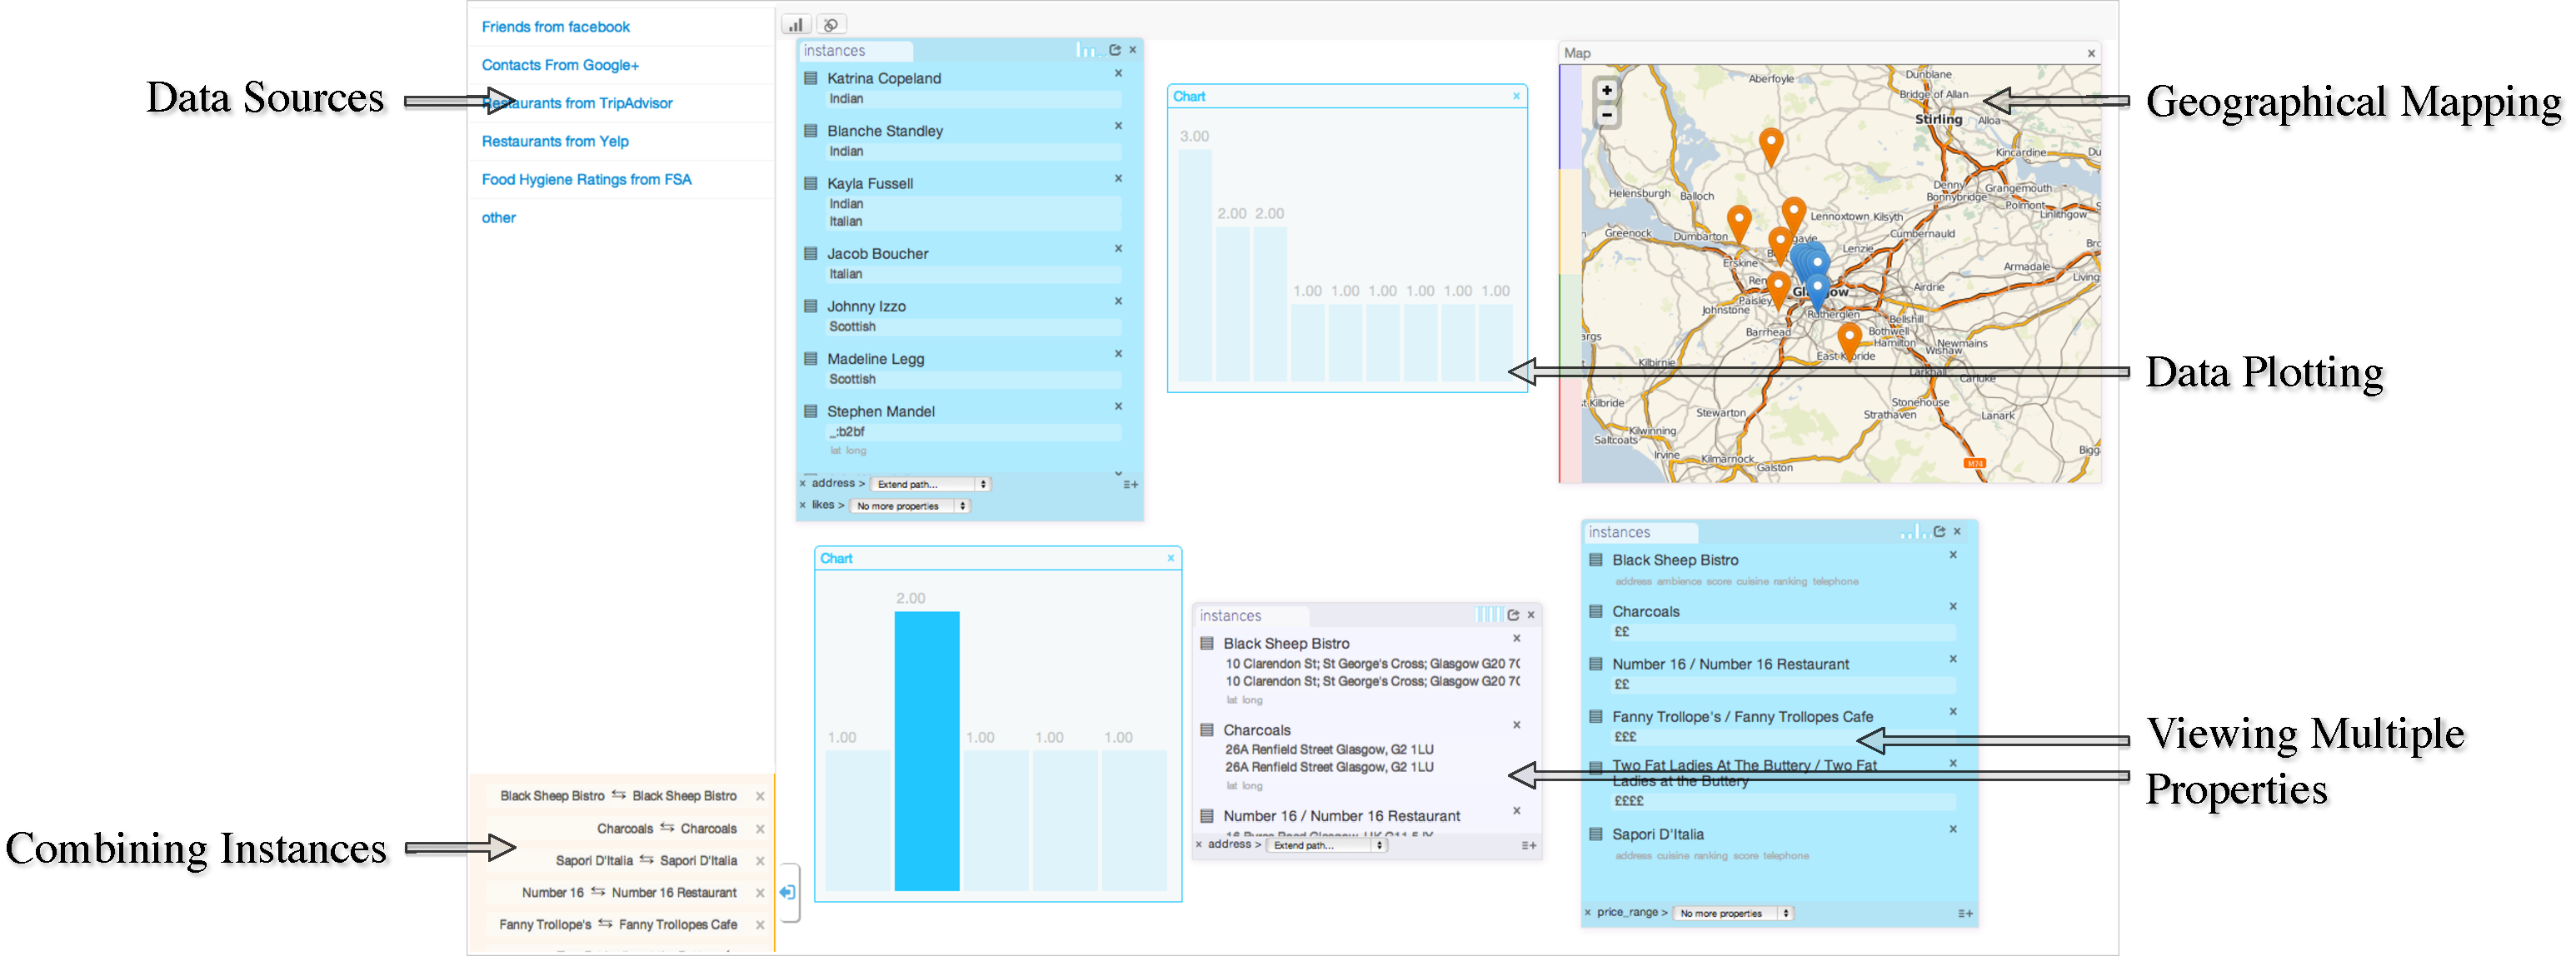
\includegraphics[width=18cm]{img/screenshot}
\caption{DataPalette Workspace, a file manager-inspired Drag and Drop interface for structured data mixing. Collapsable displays of data sources are listed on the left, from which instances or entire sets of items can be dragged to form a windoow (group) on the workspace.}
\label{fig:workspace}
\end{center}
\end{figure*}

At a high level, the overall goal of DataPalette was to empower end-users to mix arbitrary structured data feeds on-the-fly while solving their particular information task(s) - be them sensemaking or decision-making related - in order to more effectively accomplish these tasks.  Unlike Mashup makers, including Yahoo Pipes!, the goal was to facilitate such integration without a need for an explicit separate mapping or integration step, which would detract from the overall usability or usefulness of the system by making people do something that did not immediately contribute to their resolving their need.

The two prestudies provided valuable insight towards this goal that allowed us to guide our design process. The first prestudy confirmed the need for data integration by showing that people did, in fact, prefer to rely upon multiple sources of information for making important decisions, and identified the kinds of sources people most commonly used.  The second prestudy revealed that the most common inconisistencies that occurred in the APIs and data feeds available through from such data sources consisted predominantly of the simpler kinds of heterogeneity - terminological and simpler forms of structural heterogeneity, rather than the delicate semantic/modeling variety, which were comparatively rare. This gave us optimism that an interactional approach optimised around the these simpler kinds of heterogeneity would be effective.
[0
In the following sections we describe the design process we used to create prototype DataPalette, followed by a detailed description of the design of the prototype and justification.

\subsection{Process}
We followed a five-phase spiral model consisting of planning, designing, mocking-up, prototyping, and testing to derive the design of DataPalette.  This process was used because of the high degree of initial uncertainty associated with the mechanisms for facilitating the various aspects of effective data mixing that we describe in the next section. We approached this design challenge through alternative generation and elimination; alternatives were designed, drawn up and evaluated by expert colleagues (and in later iterations, non-expert potential users), who provided critiques of the alternatives. The ease with which designs could be prototyped in HTML5 with modern web frameworks allowed us to perform this develop-test-iterate rapidly through seven iterations of this process.

\subsection{Interaction with DataPalette}
In order to feel familiar to new users and focus our design efforts on integration-related aspects of the interface, we borrowed metaphors and interactions directly from MacOS Finder-style file managers.  Specifically, in the DataPalette workspace, shown in Figure \ref{fig:workspace}, the user can arbitrarily drag and drop entities from data sources (on the left) into windows that they create, resize, arrange and label. (Although the design could be generalised to supporting nested groups, our prototype only supported a single level of grouping.)

Unlike file managers, the basic unit of data is not a file, but an \emph{instance} - corresponding to an RDF instance or any small bit of structured data. In order to make working with relational graphs manageable, an early decision we made was to break up RDF-like relational data) into discrete instances with properties; for JSON or XML data feeds, we represented all subtrees with more than 1 child as its an instance.  

\subsubsection{Multipath selection: link-sliding for heterogeneous sets}

\begin{figure}[htbp]
\begin{center}
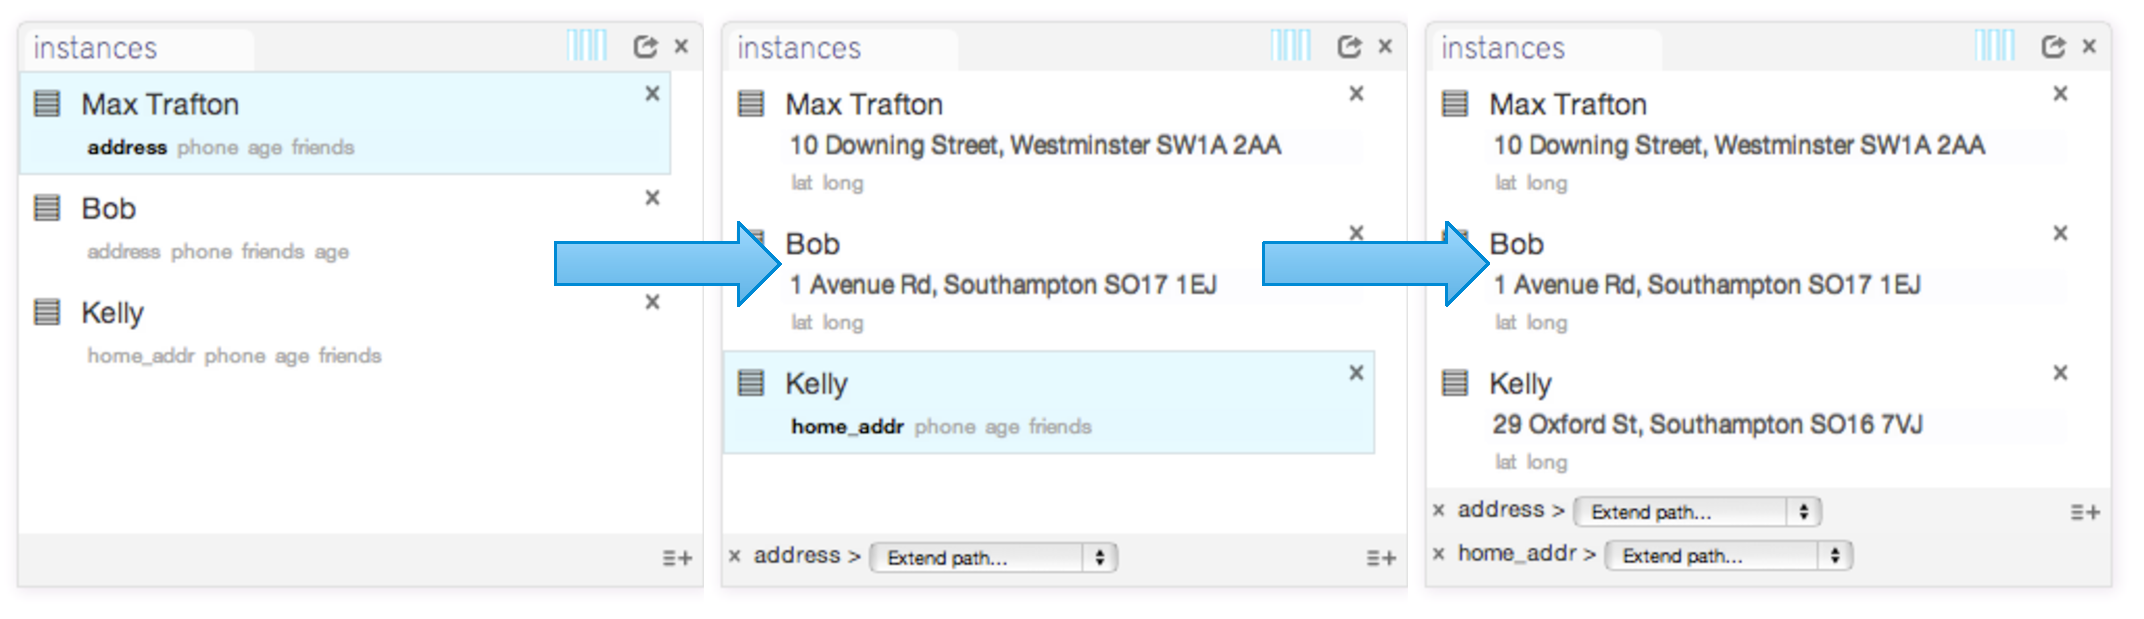
\includegraphics[width=8cm]{img/multipathing}
\caption{To see properties, users click on the name of the property. When instances do not have a particular property, additional property names can be added.}
\label{fig:multipathing}
\end{center}
\end{figure}

Typically, users are interested in viewing and comparing the \emph{properties} of instances; for example, a user might be keen to examine a product's price, rating, manufacturer and so on.  An instance's properties are displayed beneath it; selecting a property creates a \emph{path selection}, which dereferences all of the instances in a group that contain the selected property and displays their corresponding values.  For example, when a user selects the \emph{manufacturer} property for a product, all products in the same group with a manufacturer property will be dereferenced, causing the manufactueres to be displayed alongside their corresponding products.  When such a path selection is applied, the properties displayed are updated to be the set of properties of the \emph{terminating value of the path}, so that this value can be dereferenced further.  For example, once selecting a manufacturer, a user may want to know the product's manufacturer's reputation and selects their ``reputation score'' property, causing the previous path selection to be extended. This process is illustrated in Figure \ref{fig:multipathing}.

When instances cannot be dereferenced by the chosen path selection, an additional path selection can be created. As with the first path selection, it causes all matching instances to be dereferenced.  Each group can carry an arbitrary number of path selections, and each path selection can be extended continually by selecting successive properties of values. This achieves the ability to \emph{link slide} as introduced by Parallax~\cite{parallax}, but across sets of heterogeneous items by supporting multiple parallel dereferenced paths simultaneously.  

Multiple selection group-dereferencing results in two effects: 

\begin{enumerate}
\item Clicking on a property dereferences all corresponding values makes it easy to quickly compare all instances that have the same structure.  Although we were concerned that users might be surprised that path selection applied to all objects within each group in parallel, users adapted very quickly and used this functionality to save them time.   

\item Supporting dereferencing along different paths \emph{by structure} allows instances with different property names, and even sub-structures to be quickly consolidated by separate dereferencing, thereby effectively coping with terminological and structural hetereogeneity.
\end{enumerate}

\subsubsection{Coreference consolidation: Drag-and-Drop Same-as}

\begin{figure*}[htbp]
\begin{center}
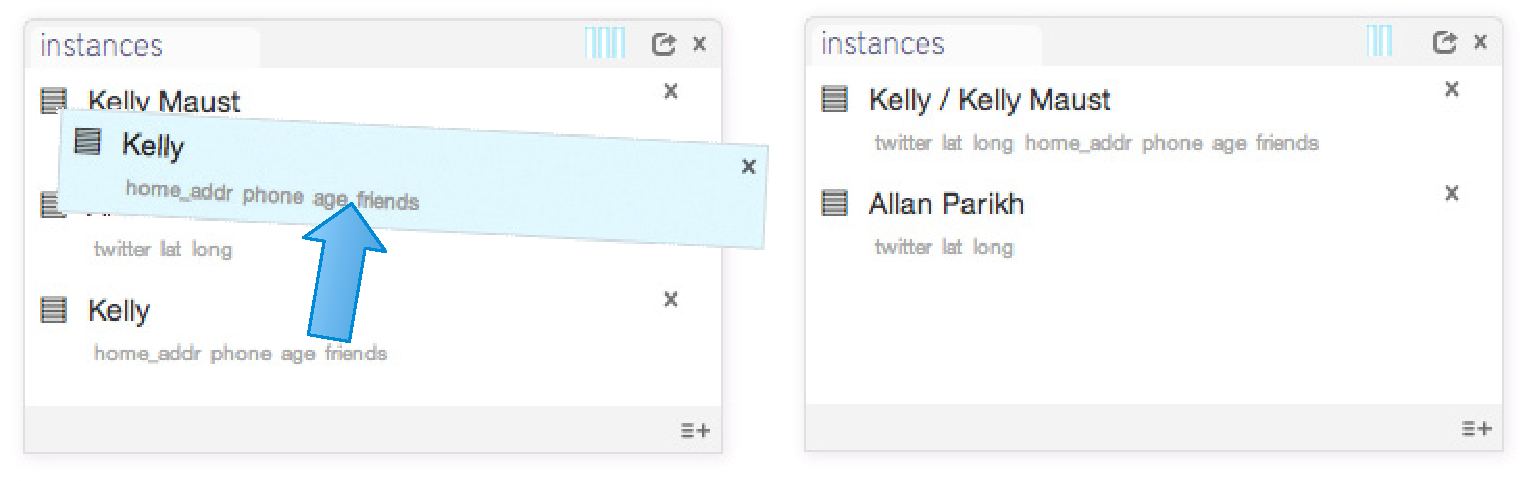
\includegraphics[width=18cm]{img/sameas}
\caption{\emph{Coreference consolidation with drag-and-drop Same-As} - When two instances represent the same entity, users can drag one on top of the other, and they are combined - effectively displaying the union of properties of both source entities. This can be un-done by deleting the Same-As relaitonship in the view in the lower-left corner of the workspace.}
\label{fig:sameas}
\end{center}
\end{figure*}

A major challenge with integration from multiple sources is coreference consolidation, or combining representations that co-refer to the same entity into one.  For example, consolidating one's friends from Facebook, Google+, and LinkedIn, one might quickly want to de-duplicate and combine friends that use multiple services so that they each have one representation.

Although we considered a way to do this automatically, PS.2 revealed no way to reliably identify co-referring instances; due to a lack of standard URIs across social networks, identifiers used by each network were system-specific and inconsistent. Thus, we sought to make instead make it user-driven, and easy to do manually.  

To remain consistent with the drag-and-drop interactions used throughout the interface, we introduced the ability to simply drag one instance on top of another to specify that two things should be combined.  This action also caused the \emph{same-as display} in the lower left of the screen to display this new combination relationship.  The display also acted as a mechanism to delete/undo combinations, which reverted representations of instances back to their original, separate forms. An illustration of this interaction is provided in Figure \ref{fig:sameas}. Although general, this can be tedious for groups of items.  Thus, to support more efficient combination, we extended this to allow entire groups to be dropped on other groups.  When this is done, DataPalette attempts to identify matching pairs among items in the dragged and target groups by comparing each pairs' labels.  Only exact matches (modulo white space/underscores) are considered matches and automatically combined.  The rest are added to the target group as distinct elements, and may be explicitly combined by hand.  We are considering more sophisticated / less fragile approaches to matching in the future, which would make the system assistive. 

By making such consolidation user-driven, we gave the user freedom to combine things when it suited him or her. As we saw in the system evaluation, while in certain circumstances users preferred combining representations, in others people preferred to keep things separate.  Thus, user-initiated consolidation afforded an additional flexibility that was ultimately deemed beneficial.

\subsubsection{Enumerated-type value consolidation}

Related to the concept of co-reference, PS.2 revealed that enumerated values of properties were often inconsistent, e.g. ``Casual dining'' vs ``Relaxed'' for a restaurant's ``atmosphere'' property. To reconcile and consolidate corresponding values from diffeent  datasources, we extended the drag and drop support of co-reference combination to also allow users to drag and drop to combine enumerated literal values as well.  

\subsubsection{``Do What I Mean'' Visualisation}

To make it easier for people to quickly visually compare aspects of instances, we created a charting tool and integrated a mapping feature.  To make these tools suitable for fast use, e.g. data exploration, we designed these tools to automatically configure display parameters instances or groups of were dropped on them, rather than making users manually specify them. In the current prototype, the DWIM behaviour of the chart automatically sets whether the plot is a histogram representation (counts of values) or numeric value display based upon the types of the dereferenced values being plotted; values that are non-numeric are counted, while numeric values are displayed.    Similarly, the map was made to detect address strings and latitude/longitude pairs, geocoding them where appropriate, and determining the optimal bounding box to display all items at maximum zoom.

\subsubsection{Model-based brushing}
Since it can get confusing having a single instance represented across several groups, we provided \emph{universal brushing} across the interface; hovering over any representation of any instance (an instance block, a map marker or a histogram bar), causes all other visible representations of that instance to lightly glow, so that the user can quickly identify all the places that a single instance is represented

% Data sources were represented as collapsable panels in a sidebar on the left of the workspace, from which instances or entire data sources could be ``pulled off'' onto the workspace.  Figure \ref{fig:workspace} displays the entire UI overview.

%% it would be nice if we had space to summarize but i fear we don't

%% \subsection{Summary of interaction capabilities}
%% \begin{itemize}
%% \item \emph{Group multi-path value selection} - Selecting any of the %% properties of an instance in a group (window) causes all of the rest %% of the instances that have that property in that group to be %% dereferenced along the same property, displaying the resulting value %% underneath the instance label.  Selecting a further property of the %% resulting value further dereferences this value.
%% \item \emph{Drag-and-drop coreference / value combination} - In order %% to specify that two instances correspond to the same entity, they can %% be simly dragged together
%% \item \emph{Group-based Drag-and-drop matching} - In order to specify %% that two instances correspond to the same entity, they can be simly %% dragged together
%% \item \emph{Universal model-based brushing} -
%% \end{itemize}

\section{Evaluation}

In order to determine whether the interaction affordances introduced in DataPalette (henceforth DP) allow users to perform serendipitous data mixing on real data feeds by end-users, we devised a within-subjects A-B trial lab study which we describe next.

\subsection{Methodology}

We first describe our methodology, starting with the three hypotheses we set out to test. These hypothesis pertain to the usability of DP by end-users (h1), whether DP achieves its stated goal of enabling end-users to integrate data (h2), and finally if it has an effect on task performance (h3) - either in how well people perform a task, how quickly they perform it, or if it reduces task effort, as follows:


% heather: instead of these low-level hypotheses, i've made higher level ones that we can explicitly address in the disucssion section - the more hypotheses we have, the more we have to come back to them; since we're short on space we might as well keep it simple!

%% Interaction-method specific hypotheses
%% \begin{itemize}
%% 	\item h1.1 - Do people understanding the problem of %% co-reference, and the need to reconcile coreference problems?
%% 	\item h1.2. Does the ability to do drag + drop combination for %% co-reference reconciliation effectively solve this problem?
%% 	\item h2.1- Do people understand the problem of structural %% differences in data?
%% 	\item h2.2 - Does multipath selection let people effectively %% deal with this -- and work with collections of heterogeneous items?
%% \end{itemize}
%% Are these interaction methods sufficient to perform common tasks %% involving heterogeneous data sources?  Does supporting these simple %% techniques facilitate task completion?

\begin{itemize}
\item \emph{h1 -} People understand how to use DP.
\item \emph{h2 -} People can effectively mix heterogeneous data with DP.
\item \emph{h3 -} Use of DP improves or facilitates task performance
\end{itemize}

\subsubsection{Study and task design}
To test these hypotheses, we designed a within-subjects lab-based A-B study in which participants were asked to perform two of four possible predefined tasks (depending on condition), with either DP (``condition A'') or a baseline interface (``condition B'') in 2 separate timed trials.  Each participant was asked to use DP for one of the trials and the baseline interface for the other; conditions were fully counterbalanced among particiants to eliminate inadvertant ordering and task bias.  

% why? why were these tasks selected? can we drop the phrase ``multi-dimensional subjective choice task'' and refer back to PS.1 to justify the choice of tasks?
The tasks were to select a restaurant for an event or university at which to study, out of six possible choices  around four possible tasks shown in Table \ref{tab:studyfactors}.  

\subsubsection{Task preparation}
% how data was prepared for each of the tasks; exactly how the A condition was done (full screen DP in a web browser, no outside access to apps),  B condition and why
We selected a shortlist of six because it is typical for users to narrow down their options to a limited selection before analysing the details of their final choices. The shortlist of universities and restaurants were taken from the top six ranked from the Complete University Guide (for task 1 and 2), Tripadvisor (for task 3) and Yelp (for task 4).  The top six were chosen from these websites because they provide a realistic shortlist and are comparable in terms of rankings and properties. The web sites used as data sources were chosen because they are the most popular and contain comparable statistics for universities and restaurants.

% why was the B condition set up this way? What did we seek to achieve?
The control (B) conditions were in a prepared Mac comprised of a web browser pre-loaded with a page with links to four live web sites, and an open instance of Excel with a workbook open containing spreadsheet versions of the same data as were loaded into DP for the A condition versions of the same tasks.  Other Office applications were also available for use and participants were allowed to visit other sites than the prespecified ones.  The purpose of this condition was to understand how people using standard desktop office software

\subsection{Data Collection}
Each study was overseen by a facilitator and an observer:  the role of the facilitator was to explain the study's protocol to the participant and to answer any questions; and the role of the observer was to observe without interacting with the user, and to take notes.  During the lab study, we recorded the audio and the participant's actions on screen. We asked the participants to follow a \emph{think-aloud} protocol as they worked, so that we could understand the reasoning behind their actions.  At the end of the study, the participant completed an exit survey.   

% In each trials, participants were given a paper notepad and pen to use if they wished.  Screen capture software recorded all interactions with applications.  Participants were asked to follow a \emph{think-aloud} protocol as they performed each task, and audio recordings (synchronized with the screen recordings) were taken. 

% This goes in results: 
% The studies lasted 40 minutes, on average.  
Both the facilitator and observer were trained on the purpose of the study, their role and how they could and couldn't influence the study.  The studies were run over 4 days.  At the end of each day the facilitators and observers met to discuss the studies' data and to revisit protocols, if necessary.


\subsection{Participant recruitement}
We recruited participants through adverts posted near the University campus and e-mails to student mailing lists.  We screened participants to be at least 18 years of age, but did not filter or preferentially select particpants based on any other criteria.  We took the first 20 that signed up and that successfully specified time slots that were available.   As described below in results, we ended up getting a large number of international students, who had varying proficiency in English.  Since all such participants had passed the requisite proficiency tests to enrol at University, we did not think this would substantially impact results.

\subsection{Task Design}

\begin{table*}[t]
\begin{center}
\small
\begin{tabular}{|p{4cm}|p{6cm}|p{6cm}|}
\hline
Task	 &Choices	&Data Sources\\
\hline
1) Three universities they would apply to study Sport Science & Universities: 1) Loughborough,  2) Durham,  3) Exeter, 4) Edinburgh, 5) Birmingham, and 6) Bath & http://www.thecompleteuniversityguide.co.uk/, http://www.ucas.ac.uk/, http://unistats.direct.gov.uk/, http://www.timeshighereducation.co.uk/world-university-rankings/ \\
\hline
2) Three universities they would apply to study History & Universities: 1) Cambridge, 2) London School of Economics and Political Science, 3) Durham, 4) Oxford, 5) St Andrews, and 6) University College London & http://www.thecompleteuniversityguide.co.uk/, http://www.ucas.ac.uk/, http://unistats.direct.gov.uk/, http://www.timeshighereducation.co.uk/world-university-rankings/ \\
\hline
3) Restaurant they would book for 12 friends in Cambridge&Restaurants : 1) Alimentum, 2) Gardenia Restaurant, 3) The Cambridge Chop House, 4) Al Casbah, 5) Midsummer House Restaurant, and 6) Nando's Restaurant. & www.yelp.co.uk, www.tripadvisor.co.uk, http://ratings.food.gov.uk/, facebook and google plus.\\
\hline
4) Restaurant they would book for 12 friends in Glagow & Restaurants :1) Black Sheep Bistro, 2) Charcoals, 3) Number 16 Family Restaurant, 4) Fanny Trollopes Cafe, 5) Two Fat Ladies At The Buttery, and 6) Sapori D'Italia. & www.yelp.co.uk, www.tripadvisor.co.uk, http://ratings.food.gov.uk/, facebook and google plus.\\
\hline
\end{tabular}
\end{center}
\caption{Tasks, choices and data sources} \label{tab:studyfactors}
\normalsize
\end{table*}%

Each task had an A and B condition.  The A condition, the participant could only use DataPalette to make their decision; and in the B condition the participant was given the choice to using any websites they desired and or workbook in Microsoft Excel containing the data taken from the data sources to make their choice on individual spreadsheets.

Each study consisted of two tasks, one A and one B condition.  Each participant was given 10 minutes to complete a task.  In order to select which tasks the participant was given, we used a latin square to permutate the tasks and conditions.  In order to train the user on how to use our interface, they viewed a five-minute DataPalette tutorial video introducing its basic functionality, how to use histograms and maps, and linking instances.

\subsection{Data Analysis}

During the data collection we collated a spreadsheet summarising the participant's gender, typical daily computer usage, the tasks allocated and basic actions performed during the task.  After we had collected the study's data, we performed our data analysis. 

TODO look further into types of data analysis....


\section{Results}

We recruited 20 participants (10 female) from the University of Southampton's international student mailing list.  All of the participants spoke English, and for 12 of them, English was not their first language.  Predominately the participants were studying various levels of Computer Science, and 5 of which studied other subjects. 

The information in Table \ref{tbl:data} was captured during the studies, so that we could statistically analyse the features used by the participants.

\begin{table*}[htdp]
\small
\begin{center}
\begin{tabular}{|r|p{0.3cm}|p{0.3cm}|p{0.3cm}|p{0.3cm}|p{0.3cm}|p{0.3cm}|p{0.3cm}|p{0.3cm}|p{0.3cm}|p{0.3cm}|p{0.3cm}|p{0.3cm}|p{0.3cm}|p{0.3cm}|p{0.3cm}|p{0.3cm}|p{0.3cm}|p{0.3cm}|p{0.3cm}|p{0.3cm}|}
\hline
Participants & 1 &2&3&4&5&6&7&8&9&10&11&12&13&14&15&16&17&18&19&20\\
\hline\hline
gender&f&m&f&f&f&f&f&m&f&f&m&f&m&f&m&m&m&m&m&m\\
A condition first task &y&y&y&n&n&y&n&n&y&y&n&n&y&y&n&n&n&n&n&n\\
\hline\hline
A Condition: task &4&2&3&4&3&&2&1&4&1&4&1&3&2&3&2&1&4&3&2\\
paper used&n&n&n&n&n&n&y&n&y&y&n&y&n&n&y&n&n&n&n&n\\
charts used &1&2&2&0&2&4&5&0&0&0&2&3&2&0&0&0&3&3&4&1\\
maps used &1&1&2&2&2&1&1&0&1&0&1&1&2&1&0&1&0&0&2&1\\ 
same as &4&3&3&6&0&2&0&2&1&0&6&5&6&2&7&0&6&7&7&7\\
number data sources  &4&3&4&4&4&3&4&3&4&4&3&3&5&4&5&4&4&5&5&4\\
chosen restaurant/uni &4.1&2.4&3.5&4.3&3.3&&2.4&1.4&4.2&1.6, \newline 1.3, \newline 1.2& 4.2& 1.4, \newline 1.5, \newline 1.3& 3.2& 2.1, \newline 2.3, \newline 2.6& 3.5, \newline 3.3&2.6, \newline 2.3, \newline 2.5&1.6, \newline 1.5, \newline 1.3&4.1&3.3&2.4, \newline 2.5, \newline 2.6\\
\hline\hline
 B Condition:task &3&&4&3&4&2&1&2&2&3&2&3&1&4&1&4&2&2&1&3\\
 paper used &n&n&n&n&n&n&y&n&y&y&n&y&n&y&y&n&n&y&n&n\\
 spreadsheet/website&&&&&&&&&&&&&&&&&&&&\\
 number of spreadsheets used&5/5&4/4&2/5&1.5&2/5&5/5&4/4&2/4&3/4&&2/4&4/5&2/4&4/5&2/4&2/5&4/4&4/4&0&5/5\\
 number of websites used&1&1&4&3&3&0&2&3&2&&1&2&3&1&2&3&2&0&4&0\\
 chosen restaurant/uni&3.5&&4.2&3.3&4.3&2.1&1.4, \newline 1.2, \newline 1.6&2.1&2.3, \newline 2.6, \newline 2.5&3.5&2.2, \newline 2.3, \newline 2.6&3.5&1.1&4.1&1.6&4.2&2.6, \newline 2.3, \newline 2.5&2.3, \newline 2.5, \newline 2.6&1.1, \newline 1.3,  \newline 1.4&3.5\\
 \hline
\end{tabular}
\end{center}
\caption{Participants data.} \label{tbl:data}
\normalsize
\end{table*}

In the A condition, where participants used DataPalette to complete their tasks they used it to collate the data on-screen, and compare multiple values directly. About half of the observed users actually used the instance combination feature of DataPalette, with the other half able to successfully make decisions without using it. Those who tried to use it were largely successful, and were able to therefore use the global brush-highlighting to simultaneously compare different statistics. Most users instantly opened up all data sources into individual boxes, in order to determine which sources contained specific statistics. The result of this technique is that the users instantly filled their screen, and ran out of space for plots and maps.

In the B conditions, participants were given the option of using websites and or a spreadsheet to make their choice.  Participants who opted to use websites to make their decisions repeatedly encountered a number of difficulties and issues. In particular, there was significant confusion over the meaning of data points, for example the percentage-based rankings of university teaching by the Times Higher Education. There were numerous usability issues in using websites, particularly in searching for university courses and course requirements. Similarly, participants found it difficult to understand the locations of restaurants in cities that they were not familiar, and could not find a way to plot the shortlist of restaurants onto the same map using the websites. Overall, the users that spent the most time using websites exhibited significant frustration attempting to locate and compare different criteria (such as course entry requirements, or restaurant locations), and all ended up falling back to using the supplied spreadsheets.

Participants who opted to use the spreadsheet to support their decisions switched between worksheets to view data from different websites.  They used different approaches to using the spreadsheets, some participants were keen to collate all data onto a single sheet, so that they could compare the values all at once. However, this approach was error prone, for example participants noticing too late that the ordering of rows was different on each sheet, so that their pasted values were incorrectly mapped. Others used pen and paper to collate the values, which was often faster and resulted in less observed frustration. While the majority of users did not
attempt anything complex with Excel (in fact only one user used charts), there was some advanced use of Excel observed.
One user explained that they did not like to look at numbers, and so coloured the cells of the types of restaurant, and the
friends' preferences, and matched the colours to make their decision. Another user calculated their own weighted metric
of which university to choose by averaging different metrics supplied by the data sources.

Notably, a number of users admittedly introduced their own bias into the choices in both A and B conditions: ``I prefer Indian food, so I will choose the Indian restaurant'', and one participant spent time on Google Maps looking at the routes to each restaurant, and eliminating those that required bus transfers (the protocol did not mention routing/transfers at all).

In the exit survey, the users noted that they would use DataPalette for finding a property to rent/buy, choosing a job and purchasing electronic devices, in the future.  However, one participant said that they would not use it for things like deciding on a restaurant because ``it would cheapen the experience'' by removing the spontaneity, but would use it for making more important decisions.  In order to improve our solutions the participants suggested making the origin of the information clearer, sorting instances, and explanations of ratings and scoring systems (however some of these are not transparent on websites).

\section{Discussion}

\subsection{Better Supporting the Task}

- are people more thorough
- do they evaluate more sources

\subsection{Causing Less Frustration}

- Gave up with aspects of the tasks later / not at all
- With websites, users gave up on websites and moved on early

\subsection{Keeping an Open Mind}

- Did users rule out choices less/later
- Did that mean they chose "better" options

\subsection{What method did people use?}

- Processes
- Organisation of data/screen
- A vs B, how are they different?


% DAN's  qual analysis of processes

In order to complete the tasks, the users followed a number of different processes. The most common process followed
was {\it collation} of data, either on-screen or on paper. Some users were proficient enough to copy and paste data
in the supplied spreadsheets from worksheet to worksheet, while others manually typed data value-by-value across worksheets.
Others preferred to collate the data from screen to paper, in order to compare multiple data points. A similar process that
some participants followed was to determine which values of a particular statistic were acceptable, and keep a paper tally
of these next to the set of choices. They then made their choice based on the value of this tally.

Two contrasting approaches that participants followed was to use the data to rule out candidates, or to use the data to
directly compare candidates at once. Our pool of participants exhibited both behaviours evenly, however in the condition
when using the DataPalette interface, significantly more comparison (and visualisation of values) was performed, with fewer
participants using the ``ruling out'' process. A consequence of this was that when asked to justify their choices, users were
able to verify their values on-screen immediately, whereas those who had ruled-out had to memorise their reasons, with
mixed success  -- many participants had to look through the data sources to re-find the reasons why they has ruled out some choices.

Therefore, the uses that were using DataPalette were more confident in their choices, and knew exactly why they had chosen them,
often pointing to the screens to show and verify each choice as they explained them.

\subsection{}

- data integration literature demands 'correct' but perfect is the enemy of the good.


%What we found 
%
%What we didn't find (evidence for)
%
%What we might look at next -- follow-on work
%		We focused on terminological heterogeneity -- didn't address structural heterogeneity, semantic heterogeneity
%		We focused on finite (small) sets Streaming data (how do select future data --) 
%		Scale - small data, what are the facilites required for large data
%		Collaborative - how might interaction support multiple users collaborating?
%
%Limitations found from study... what is the take away from the limitations









\section{Conclusion} %Key findings of the whole paper and its implications

% ``perfect'' be the enemy of the good

%% In this paper, we take the position that there is a need for a difference in focus between the approaches taken to data integration between the approaches taken in database integration and that of PIM, because of vast differences in requirements.  In database systems, the overall objective is usually to allow multiple large databases to be accessed as if one. This requires essentially full mapping of all data types and objects and well-defined semantics concerning where and how data gets converted. The upfront costs of such complete integration are typically high, but are typically justified in the long-term, high-volume use cases imagined. In typical sensemaking scenarios of PIM, however, people might need to combine information from multiple sources for a one-off task; meaning that any upfront cost would directly impact the time and effort a person has allocated for their task.  Moreover, while a fully, uniform query capability might be nice, such capability is likely of less overall importance for a single quick task than simply being able to quickly and easily identify and cope with differences.

Just as journalism became peer-produced with the explosion of blogging, data journalism is on the brink of moving from skilled data analyists the likes of The Guardian Datablog staff\footnote{Guardian Datablog - \url{}} into the hands of the ordinary citizen \cite{datajournalismhandbook}.  In order for this to happen, however, tools that allow people to effectively combine data more effectively than current structured PIM tools and generic spreadsheet tools will become increasingly important. 

\section{Acknowledgments}


% Balancing columns in a ref list is a bit of a pain because you
% either use a hack like flushend or balance, or manually insert
% a column break.  http://www.tex.ac.uk/cgi-bin/texfaq2html?label=balance
% multicols doesn't work because we're already in two-column mode,
% and flushend isn't awesome, so I choose balance.  See this
% for more info: http://cs.brown.edu/system/software/latex/doc/balance.pdf
%
% Note that in a perfect world balance wants to be in the first
% column of the last page.
%
% If balance doesn't work for you, you can remove that and
% hard-code a column break into the bbl file right before you
% submit:
%
% http://stackoverflow.com/questions/2149854/how-to-manually-equalize-columns-
% in-an-ieee-paper-if-using-bibtex
%
% Or, just remove \balance and give up on balancing the last page.
%
\balance

% If you want to use smaller typesetting for the reference list,
% uncomment the following line:
% \small
\bibliographystyle{acm-sigchi}
\bibliography{carpedata}
\end{document}
